\documentclass{article}
\usepackage[utf8]{inputenc}
\usepackage{listings}
\usepackage{float}
\usepackage{algorithm}
\usepackage{fancyhdr}
\usepackage{xcolor}
\usepackage{graphics}
\usepackage{graphicx}

\begin{titlepage}
\title{\textbf{Network Lab Exam Question 3-A}}

\author{\\ \\  Albin Antony \\ Roll No:10 \\   TVE16CS010 }
\date{25 April 2019}

\end{titlepage}

\pagestyle{fancy}
\fancyhf{}
\rhead{Lab Exam}
\lhead{Que-3A}
\rfoot{\thepage}

\begin{document}
\definecolor{lightgray}{rgb}{.96,.96,.96}
\lstset{numbers=left, numberstyle=\tiny, stepnumber=1, numbersep=5pt,frame=hidden,breaklines=true,backgroundcolor=\color{lightgray},xleftmargin=0pt,xrightmargin=-20pt}
\pagenumbering{gobble}
  \maketitle
  \newpage
  \pagenumbering{arabic}
  \section{Narrow Brigde}
  \subsection{Problem Statement}
 A city is built on two islands connected by a narrow bridge. There are many
cars driving throughout the city and occasionally crossing the bridge. The bridge is only wide
enough for traffic in one direction at a time. Because the bridge is narrow the cars must also
travel slowly while crossing the bridge (i.e. it should take some time). There is no traffic
light.
\newline
\newline

When a car decides to cross the bridge, one of three situations can occur:
\begin{itemize}
\item i) the bridge is free, in which case the car may cross.
\item ii) the bridge is occupied, and the traffic on the bridge is travelling in the right
direction, so the car is allowed to cross.
\item iii) the bridge is occupied, but the traffic is in the wrong direction. The car must either
wait until the bridge is free, or come back later and try again.
\end{itemize}
Make sure that you have enough cars, and that they decide to cross the bridge often enough
that all three of the traffic situations can occur. Use one process to represent one car.
  
  \subsection{Theory}
 \subsubsection{Thread}
 A thread is a path of execution within a process. A process can contain multiple
threads.A thread is also known as lightweight process. The idea is to achieve
parallelism by dividing a process into multiple threads.A thread is a single se-
quence stream within in a process. Because threads have some of the properties
of processes, they are sometimes called lightweight processes. Threads are not
independent of one other like processes as a result threads shares with other
threads their code section, data section and OS resources like open files and sig-
nals. But, like process, a thread has its own program counter (PC), a register
set, and a stack space
\subsubsection{Mutex}

    A Mutex is a lock that we set before using a shared resource and release after using it.
    When the lock is set, no other thread can access the locked region of code.
    So we see that even if thread 2 is scheduled while thread 1 was not done accessing the shared resource and the code is locked by thread 1 using mutexes then thread 2 cannot even access that region of code.
    So this ensures a synchronized access of shared resources in the code.

  \subsection{Algorithm}
%   algorithm file
  \begin{algorithm}[H]
  \lstinputlisting[language=c++]{algorithm/bridge}
  \caption{Algorithm for Narrow Server}
  \end{algorithm}
  
  Each car calls a thread to cross a bridge.For a car going left carleft is used and for a car going right carright is used. A counter uses count of traffic to right and left.If counter is positive cars are going left and any car going left can access the lock.If counter is negative all cars on bridge are going right.All cars going right can enter the bridge.

  \subsection{Program}
%   program file
  \lstinputlisting[language=c++,numbers=none]{code/bridge.cpp}
  \newpage
  \subsubsection{To run the program:}
   \begin{verbatim}

g++ bridge.cpp -lpthread


  \end{verbatim}
  
  \subsection{Output}
\subsubsection{Test case 1}
 \begin{figure}[H]
\centering

\includegraphics[width=400]{img/bd1.png}
\end{figure}

\subsubsection{Test case 2}
 \begin{figure}[H]
\centering

\includegraphics[width=400]{img/bd2.png}
\end{figure}

\subsubsection{Test case 3}
 \begin{figure}[H]
\centering
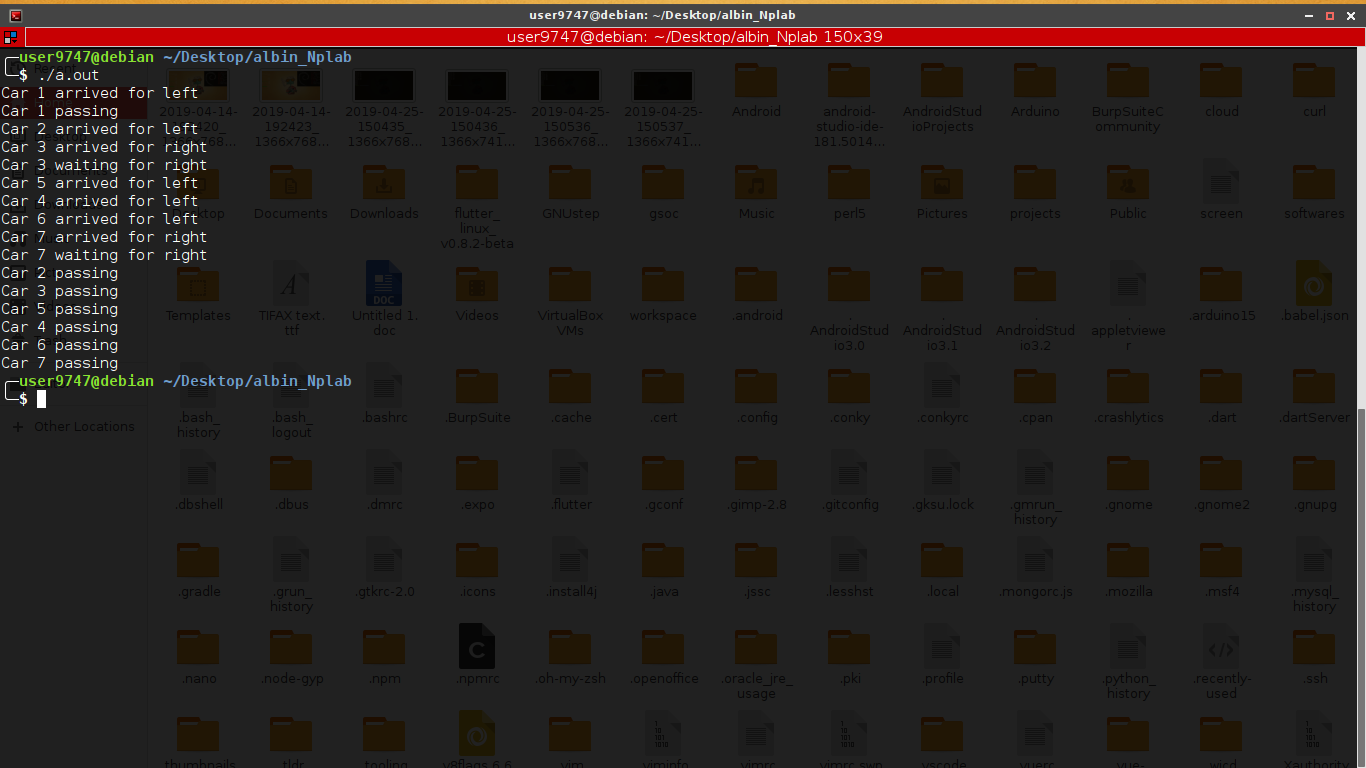
\includegraphics[width=400]{img/bd3.png}
\end{figure}
  
  
  

\end{document}